\documentclass[conference]{IEEEtran}
\IEEEoverridecommandlockouts
\usepackage{cite}
\usepackage{amsmath,amssymb,amsfonts}
\usepackage{algorithmic}
\usepackage{graphicx}
\usepackage{textcomp}
\usepackage{xcolor}
\usepackage{multirow}
\usepackage{booktabs}
\usepackage{float}
\usepackage{caption}
\captionsetup[figure]{font=footnotesize, labelsep=period, justification=centering}
\captionsetup[table]{font=footnotesize, labelsep=period, justification=centering}
\renewcommand{\figurename}{Gambar}
\renewcommand{\tablename}{Tabel}
\renewcommand{\thetable}{\arabic{table}}
\graphicspath{{../../core/gambar/}}

\def\BibTeX{{\rm B\kern-.05em{\sc i\kern-.025em b}\kern-.08em
    T\kern-.1667em\lower.7ex\hbox{E}\kern-.125emX}}

\begin{document}

\title{Implementasi Federated Learning pada Sistem Kehadiran Berbasis Pengenalan Wajah di Lingkungan Edge Computing}

\author{
    \IEEEauthorblockN{Steven Figo\textsuperscript{1}, Fuad Dary Rosyadi\textsuperscript{2}, Rizka Wakhidatus Sholikah\textsuperscript{3}}
    \IEEEauthorblockA{Departemen Teknologi Informasi, Fakultas Teknologi Elektro dan Informatika Cerdas \\
    Institut Teknologi Sepuluh Nopember, Surabaya, Indonesia \\
    Email: \textsuperscript{1}stevenfigo72@email.com, \textsuperscript{2}rosyadi@its.ac.id, \textsuperscript{3}wakhidatus@its.ac.id}
}

\maketitle

\begin{abstract}
Sistem absensi berbasis pengenalan wajah saat ini telah banyak diterapkan untuk mengotomatiskan pencatatan kehadiran, namun metode konvensional berbasis Centralized Learning mengharuskan pengumpulan citra wajah mentah ke server pusat yang rentan terhadap risiko kebocoran data biometrik sensitif serta pemborosan bandwidth jaringan. Penelitian ini mengusulkan implementasi Federated Learning menggunakan algoritma FedProx dan model MobileFaceNet yang dikontainerisasi dengan Docker untuk membangun sistem kehadiran terdistribusi pada lingkungan Edge Computing menggunakan perangkat keras heterogen (Jetson Nano dan Raspberry Pi 3 Model B). Pendekatan ini memungkinkan proses pelatihan model dilakukan secara lokal pada masing-masing perangkat edge tanpa mengirimkan data biometrik mentah mahasiswa ke server, sehingga privasi data tetap terjaga secara maksimal. Pengujian dilakukan melalui evaluasi performa model pelatihan, efisiensi sumber daya, serta pengujian inferensi nyata (real-life) dan video simulasi. Hasil penelitian menunjukkan bahwa model global hasil Federated Learning mampu mencapai tingkat akurasi sebesar 98,16\% dengan validation loss 0,3599, yang berhasil menyeimbangi akurasi Centralized Learning sebesar 96,93\%. Selain itu, metode terdistribusi ini sangat efisien dalam penggunaan bandwidth jaringan dengan hanya mentransmisikan data sebesar 159,46 MB, jauh lebih hemat dibandingkan metode terpusat yang menghabiskan 1152,34 MB. Pada pengujian inferensi nyata, sistem mencatatkan keberhasilan fungsionalitas 100\% pada jarak 0,5 hingga 3 meter pada kondisi cahaya cukup dan minim dengan akurasi klasifikasi stabil di atas 90\% menggunakan ambang batas kepercayaan 0,7. Adapun latensi inferensi lokal pada Jetson Nano berjalan cepat ($\sim$700 ms) sedangkan Raspberry Pi berjalan lebih lambat ($\sim$3100 ms) akibat keterbatasan kapasitas RAM. Penelitian ini menunjukkan bahwa integrasi Federated Learning dan Edge Computing sangat efektif dalam mengoptimalkan sistem presensi yang aman, responsif, dan hemat bandwidth.
\end{abstract}

\begin{IEEEkeywords}
Edge Computing, Face Recognition, Federated Learning, MobileFaceNet, Smart Attendance.
\end{IEEEkeywords}

\section{Introduction}
Perkembangan kecerdasan buatan (AI) dalam beberapa tahun terakhir berlangsung sangat pesat dan memberikan dampak signifikan pada berbagai sektor seperti industri, pendidikan, kesehatan, dan transportasi. Kemampuan AI dalam mengolah data dalam jumlah besar serta menemukan pola tertentu membuat proses pengambilan keputusan menjadi lebih cepat dan akurat. Di saat yang sama, penggunaan perangkat Internet of Things (IoT) juga semakin meluas sehingga menghasilkan lebih banyak data dari perangkat yang saling terhubung. Namun, perkembangan AI dan IoT ini menghadirkan tantangan baru, terutama terkait keamanan data, privasi pengguna, dan kompleksitas dalam pengelolaannya \cite{b1}.

Sebagian besar sistem AI masih menggunakan metode Centralized Learning, di mana seluruh data dikumpulkan ke satu server pusat untuk dilatih. Pendekatan ini memang efektif, tetapi kurang ideal karena berpotensi menimbulkan kebocoran data pribadi serta memerlukan bandwidth yang besar, terutama ketika data mentah dikirim dari banyak perangkat IoT \cite{b2}. Permasalahan ini menjadi semakin menonjol pada aplikasi yang memanfaatkan data biometrik, seperti pengenalan wajah, karena jenis data tersebut sangat sensitif dan tidak dapat diganti jika terjadi kebocoran.

Pengenalan wajah merupakan salah satu teknologi yang banyak digunakan dalam sistem kehadiran karena mampu mengotomatiskan proses identifikasi dan mengurangi ketergantungan pada metode absensi manual. Namun, penggunaan citra wajah sebagai data biometrik menimbulkan persoalan penting terkait privasi, terutama ketika data perlu diproses atau disimpan di server pusat. Dalam Penelitian \cite{b3} mengembangkan sistem kehadiran berbasis convolutional neural network (CNN) yang dijalankan pada perangkat edge seperti Raspberry Pi and Jetson Nano, di mana proses inferensi dilakukan secara lokal untuk membatasi pergerakan data sensitif. Meskipun demikian, proses pelatihan model pada penelitian tersebut masih dilakukan secara terpusat sehingga data wajah tetap harus dikumpulkan ke server ketika pembaruan model diperlukan. Hal ini menunjukkan bahwa isu privasi pada tahap pelatihan belum sepenuhnya teratasi.

Untuk mengurangi ketergantungan pada pelatihan terpusat, Federated Learning diperkenalkan sebagai pendekatan yang memungkinkan pelatihan model dilakukan langsung di perangkat pengguna. Dalam Federated Learning, data mentah tidak perlu dikirim ke server pusat, hanya parameter atau pembaruan model yang dikirim untuk digabungkan menjadi model global \cite{b4}. Dengan mekanisme tersebut, privasi data biometrik dapat lebih terjaga dan kebutuhan bandwidth menjadi lebih rendah. Penelitian \cite{b5} juga menunjukkan bahwa Federated Learning efektif untuk melatih model pengenalan wajah karena citra wajah pengguna tetap berada di perangkat masing-masing. Meskipun temuan tersebut menunjukkan potensi besar Federated Learning untuk aplikasi biometrik, hingga saat ini belum terdapat penelitian yang menerapkan Federated Learning pada sistem kehadiran berbasis pengenalan wajah di perangkat edge, sehingga menyisakan celah penelitian yang masih perlu dieksplorasi.

Berdasarkan permasalahan tersebut, penelitian tugas akhir ini mengusulkan penerapan Federated Learning pada sistem kehadiran berbasis pengenalan wajah di lingkungan Edge Computing. Dalam penelitian ini, model MobileFaceNet akan dilatih secara lokal di perangkat client, sehingga citra wajah tidak perlu dikirim ke server pusat. Proses distribusi dan orkestrasi server dan client akan menggunakan Docker agar sistem lebih mudah dijalankan dan direplikasi. Harapannya, kombinasi Federated Learning, MobileFaceNet, dan Edge Computing dapat menghasilkan sistem kehadiran yang lebih aman, efisien, serta tetap menjaga privasi pengguna.

\section{Tinjauan Pustaka}

\subsection{Federated Learning}
\textit{Federated Learning} merupakan paradigma pembelajaran mesin terdesentralisasi yang dikembangkan untuk mengatasi keterbatasan \textit{Centralized Learning}, khususnya terkait keamanan privasi dan efisiensi \textit{bandwidth}. Konsep dasar \textit{Federated Learning} pertama kali diperkenalkan oleh Google, di mana proses pelatihan model dilakukan langsung di perangkat lokal (\textit{client}) menggunakan data lokal masing-masing tanpa perlu mengirimkan data mentah tersebut ke \textit{server} pusat \cite{b6}. \textit{Client} hanya mengirimkan parameter model lokal (bobot atau gradien) hasil pelatihan ke \textit{server} pusat. \textit{Server} pusat kemudian mengagregasi parameter tersebut untuk membentuk model global baru, yang selanjutnya didistribusikan kembali ke \textit{client} untuk iterasi berikutnya hingga konvergensi tercapai. Pendekatan ini sangat relevan untuk menjaga privasi data sensitif seperti citra wajah, karena data biometrik tetap tersimpan aman di sisi perangkat \textit{client}.

\subsection{Flower Framework}
Dalam pengembangan sistem \textit{Federated Learning}, dibutuhkan sebuah kerangka kerja yang fleksibel dan mendukung penerapan pada perangkat \textit{edge}. Flower merupakan pustaka \textit{open-source} yang dirancang secara agnostik terhadap kerangka kerja \textit{deep learning} yang digunakan, seperti PyTorch, TensorFlow, atau JAX \cite{b7}. Flower memfasilitasi komunikasi antara \textit{server} (agregator) dan banyak \textit{client} menggunakan protokol gRPC (\textit{gRPC Remote Procedure Calls}) yang memiliki keunggulan berupa latensi rendah dan konsumsi \textit{bandwidth} yang minimal, sehingga sangat ideal untuk dijalankan di lingkungan perangkat \textit{edge} dengan keterbatasan sumber daya. Pustaka ini menangani siklus pelatihan terdistribusi, pengiriman parameter model, hingga integrasi strategi agregasi kustom.

\subsection{Algoritma FedProx}
Algoritma \textit{Federated Proximal} (FedProx) hadir sebagai bentuk pengembangan dari metode konvensional \textit{Federated Averaging} (FedAvg) untuk mengatasi kendala heterogenitas pada jaringan terdistribusi \cite{b8}. Konsep utama dari FedProx adalah restrukturisasi pada fungsi objektif lokal di setiap perangkat \textit{client} dengan menambahkan sebuah komponen penalti matematis yang disebut \textit{proximal term} ($\mu$). Mekanisme ini dirancang untuk membatasi arah pembaruan parameter selama pelatihan lokal agar tidak melenceng terlalu jauh dari arsitektur model global yang dikelola oleh \textit{server} pusat. Fungsi objektif lokal utama FedProx dirumuskan sebagai:
\begin{equation}
  \label{eq:fedprox-obj}
  \min_{w_k} \left[ F_k(w_k) + \frac{\mu}{2} \|w_k - w^g\|^2 \right]
\end{equation}

Di mana $w_k$ melambangkan representasi matriks parameter model lokal pada \textit{client} ke-$k$, $w^g$ adalah bobot model global saat itu, $F_k(w_k)$ melambangkan fungsi \textit{loss} lokal \textit{client}, dan $\mu$ menyatakan koefisien regularisasi \textit{proximal term}. Penambahan \textit{proximal term} ($\mu$) terbukti efektif menstabilkan konvergensi model global dan mencegah fenomena \textit{client drift} ketika karakteristik dataset lokal antar-\textit{client} sangat bervariasi.

\subsection{Face Recognition}
Sistem pengenalan wajah (\textit{Face Recognition}) merupakan teknologi biometrik yang berfungsi mengidentifikasi atau memverifikasi identitas seseorang berdasarkan karakteristik fisiologis wajahnya. Tahapan utama dalam pengenalan wajah meliputi deteksi wajah (menentukan posisi wajah dalam citra), penyelarasan wajah (\textit{alignment}), ekstraksi fitur (\textit{feature extraction}) untuk menghasilkan representasi vektor numerik (\textit{face embedding}), dan pencocokan wajah berdasarkan metrik kemiripan jarak (seperti \textit{Cosine Similarity} atau \textit{Euclidean Distance}) \cite{b5}. Pada implementasi presensi terdistribusi, model deteksi dan pengenalan wajah harus dijalankan secara efisien pada perangkat \textit{edge} untuk memberikan respon kehadiran secara \textit{real-time}.

\subsection{MobileFaceNet}
MobileFaceNet merupakan arsitektur \textit{deep learning} yang dirancang untuk pengenalan wajah pada perangkat dengan sumber daya terbatas \cite{b9}. Model ini termasuk jaringan ringan (\textit{lightweight CNN}) yang fokus pada efisiensi komputasi tanpa mengorbankan akurasi secara signifikan. MobileFaceNet menggunakan teknik seperti \textit{depthwise separable convolution} yang membuat ukuran model kecil namun tetap mampu mengekstraksi fitur wajah dengan baik.

Dalam penelitian ini, MobileFaceNet diimplementasikan sebagai model utama untuk pengenalan wajah pada sistem kehadiran. Penelitian ini menerapkan strategi \textit{transfer learning} dengan memanfaatkan bobot awal (\textit{pre-trained weights}) yang bersumber dari implementasi \textit{open-source} MobileFaceNet berbasis PyTorch oleh Xiaoccer \cite{b10} yang dilatih menggunakan dataset CASIA-WebFace dan dievaluasi menggunakan dataset LFW (\textit{Labelled Faces in the Wild}). Penggunaan bobot awal ini berfungsi sebagai inisialisasi dasar untuk mempercepat konvergensi sebelum dilakukan proses \textit{Federated Learning}. Model ini dipilih karena karakteristiknya yang ringan, sehingga mampu beroperasi secara optimal dan efisien pada perangkat \textit{edge} yang memiliki keterbatasan sumber daya komputasi.

\section{Metodologi Penelitian}

\subsection{Alur Penelitian}
Penelitian ini menerapkan metode \textit{Federated Learning} pada lingkungan \textit{Edge Computing} sebagai pendekatan utama dalam pembangunan sistem. Tahapan pelaksanaan penelitian, dimulai dari pengumpulan data hingga evaluasi, diilustrasikan melalui diagram alur pada Gambar~\ref{fig:diagram-alur-penelitian}.

\begin{figure*}[htbp]
  \centering
  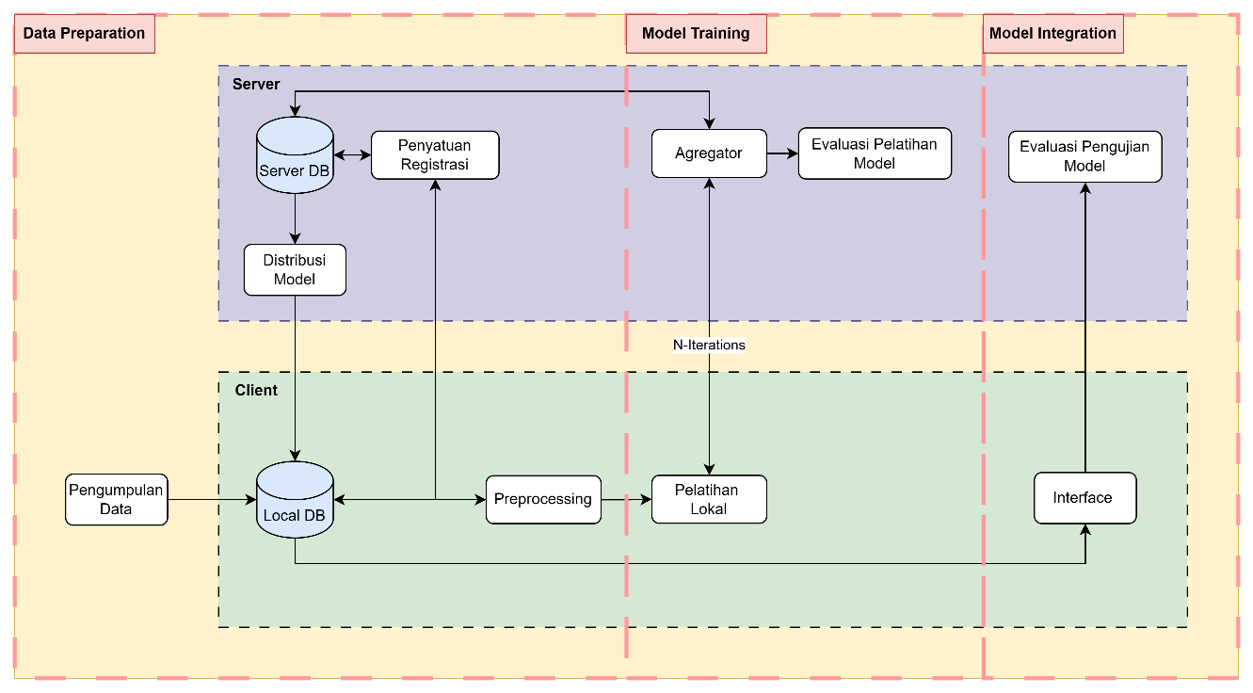
\includegraphics[width=\textwidth]{../../core/gambar/Diagram_Alur_Penelitian.png}
  \caption{Diagram Alur Penelitian}
  \label{fig:diagram-alur-penelitian}
\end{figure*}

\subsection{Pra-pemrosesan Data}
Tahap awal dimulai dengan merekam karakteristik wajah dari 30 subjek mahasiswa menggunakan \textit{webcam}. Pipa pra-pemrosesan data citra wajah di tingkat lokal dijalankan secara sekuensial melalui lima tahapan utama:
\begin{enumerate}
    \item \textit{Penyaringan Kualitas Ketajaman}: Menggunakan operator Laplacian untuk menghitung skor varians ketajaman fokus citra dan menyaring hanya 50 berkas citra wajah tertajam dari ribuan \textit{frame} yang tertangkap kamera.
    \item \textit{Deteksi Wajah dan Landmarks}: Menggunakan model MTCNN untuk mengekstrak kotak pembatas (\textit{bounding box}) serta 5 titik koordinat kanonik wajah (\textit{landmarks}) meliputi mata kiri, mata kanan, hidung, mulut kiri, dan mulut kanan.
    \item \textit{Penyelarasan dan Normalisasi Resolusi}: Melakukan rotasi citra secara afinitas dua dimensi agar wajah tegak simetris, diikuti pemotongan dan pengubahan resolusi gambar menjadi 96$\times$112 piksel.
    \item \textit{Normalisasi Nilai Tensor}: Mengonversi citra menjadi tensor PyTorch dengan penskalaan rentang nilai piksel diselaraskan pada parameter $-1$ hingga $1$ guna menjaga stabilitas pelatihan model.
    \item \textit{Enkripsi Data Biometrik}: Vektor representasi wajah (\textit{face embedding}) dienkripsi menggunakan algoritma AES-256 bit mode CBC untuk mengamankan data biometrik di penyimpanan lokal PostgreSQL \textit{client} sebelum proses transmisi.
\end{enumerate}

Untuk mensimulasikan lingkungan jaringan terdistribusi, data latih biometrik dari 30 subjek tersebut dibagi rata ke dalam dua perangkat \textit{client edge} (masing-masing menyimpan 15 subjek mahasiswa yang berbeda).

\subsection{Arsitektur Sistem}
Sistem presensi dirancang menggunakan model arsitektur \textit{client-server} yang terisolasi di dalam wadah kontainer \textit{Docker} guna menyamakan dependensi pustaka perangkat lunak. Perangkat keras lokal terdiri atas dua node \textit{client edge} heterogen:
\begin{enumerate}
    \item \textit{Client 1}: Perangkat NVIDIA Jetson Nano (Quad-core ARM Cortex-A57 @ 1,48 GHz, RAM 4 GB).
    \item \textit{Client 2}: Perangkat Raspberry Pi 3 Model B (Quad-core ARM Cortex-A53 @ 1,20 GHz, RAM 1 GB).
\end{enumerate}
Kedua perangkat terhubung dengan komputer \textit{server} pusat (vCPU 4 core, RAM 6 GB) sebagai agregator model global menggunakan kerangka kerja Flower melalui protokol komunikasi gRPC.

\subsection{Pelatihan Model}
Pelatihan model MobileFaceNet dilakukan secara terdesentralisasi menggunakan optimasi SGD dan fungsi \textit{loss} ArcFace. Siklus pelatihan dijalankan selama 10 ronde komunikasi global dengan parameter pelatihan lokal sebagai berikut:
\begin{itemize}
    \item Pelatihan lokal pada \textit{client} dibatasi sebanyak 1 \textit{epoch} per ronde.
    \item Lapisan \textit{backbone} model MobileFaceNet dibekukan (\textit{frozen}) untuk meminimalkan beban komputasi CPU \textit{client}, sedangkan pembaruan parameter hanya aktif pada \textit{embedding layer} dan \textit{classifier head}.
    \item Penambahan komponen \textit{proximal term} ($\mu = 0,04$) untuk membatasi pergeseran pembaruan bobot model lokal agar tidak menyimpang jauh dari model global (menghindari fenomena \textit{client drift} akibat data \textit{non-IID}).
    \item Agregasi model global di \textit{server} mengadopsi rata-rata tertimbang (\textit{weighted averaging}) parameter konvolusi model lokal dari kedua \textit{client} tanpa mengagregasi statistik lapisan \textit{Batch Normalization} (BN) untuk mempertahankan personalisasi tingkat \textit{client}.
\end{itemize}

\subsection{Inferensi Lokal}
Pengoperasian sistem presensi secara langsung dijalankan pada sisi \textit{client edge}. Aliran video dari kamera diolah per \textit{frame} menggunakan MTCNN untuk deteksi wajah, diikuti ekstraksi vektor fitur (\textit{face embedding} berdimensi 128) oleh model MobileFaceNet global mutakhir hasil pelatihan. Guna meminimalkan kesalahan deteksi dinamis, sistem menerapkan jaring pengaman \textit{Temporal Voting} sepanjang rentang waktu 3 \textit{frame} terakhir. Nilai vektor embedding dicocokkan terhadap \textit{head centroid} referensi identitas mahasiswa menggunakan metrik kemiripan \textit{Cosine Similarity} dengan ambang batas kepercayaan (\textit{confidence threshold}) sebesar 0,7.

\subsection{Evaluasi Sistem}
Kelayakan sistem dievaluasi secara menyeluruh dengan membandingkan model hasil pelatihan terdistribusi FedProx terhadap metode latih terpusat (\textit{Centralized Learning}) sebagai \textit{baseline}. Metrik evaluasi mencakup tiga aspek:
\begin{enumerate}
    \item \textit{Evaluasi Pelatihan}: Akurasi pelatihan model global, \textit{validation loss}, total durasi waktu latih (detik), efisiensi penggunaan \textit{bandwidth} jaringan transmisi model (MB), serta total konsumsi energi listrik perangkat (kWh) menggunakan pustaka CodeCarbon.
    \item \textit{Evaluasi Inferensi Nyata (Real-life)}: Akurasi keberhasilan klasifikasi wajah lintas \textit{client}, nilai \textit{Cosine Similarity} (rata-rata, maksimum, minimum), dan latensi inferensi lokal (ms) pada variasi jarak (0,5--3 meter) serta kondisi pencahayaan (cukup cahaya 341,01 lux dan minim cahaya 47,54 lux).
    \item \textit{Evaluasi Video Simulasi}: Total waktu pemrosesan aliran video absensi pada unit CPU \textit{client}, persentase keberhasilan pencatatan kehadiran mahasiswa terdaftar, dan jumlah kasus salah absen (\textit{false acceptance}).
\end{enumerate}

\section{Hasil dan Pembahasan}

\subsection{Pengujian Pelatihan Model}
Evaluasi performa komputasi dan karakteristik pembaruan bobot model dilakukan untuk membandingkan efisiensi sumber daya serta beban ekosistem antara metode \textit{Federated Learning} (menggunakan FedProx) dan \textit{Centralized Learning}. Perbandingan metrik antara kedua metode dirangkum pada Tabel~\ref{tab:perbandingan-pelatihan}, metrik durasi pelatihan \textit{client Federated Learning} dirangkum pada Tabel~\ref{tab:fl-client-metrics}, sementara dinamika konvergensi disajikan pada Gambar~\ref{fig:chart-fl-server}, Gambar~\ref{fig:chart-fl-client1}, Gambar~\ref{fig:chart-fl-client2}, dan Gambar~\ref{fig:chart-cl}.

{\fontsize{8}{9}\selectfont
\begin{table}[H]
\caption{Perbandingan Metrik Pelatihan \textit{Federated Learning} dan \textit{Centralized Learning}}
\begin{center}
\resizebox{\columnwidth}{!}{
\begin{tabular}{|l|c|c|}
\hline
\textbf{Parameter Evaluasi} & \textbf{\textit{Centralized Learning}} & \textbf{\textit{Federated Learning}} \\
\hline
\textit{Loss} & 4,7318 & 1,5366 \\
\hline
\textit{Accuracy} (\%) & 96,93 & 98,16 \\
\hline
\textit{Validation Loss} & 0,5457 & 0,3599 \\
\hline
\textit{Validation Accuracy} (\%) & 98,95 & 99,66 \\
\hline
Total Waktu Pelatihan (detik) & 439,99 & 5034,13 \\
\hline
\textit{Bandwidth} (MB) & 1152,34 & 159,46 \\
\hline
Konsumsi Energi (kWh) & 0,012222 & 0,089481 \\
\hline
\end{tabular}
}
\label{tab:perbandingan-pelatihan}
\end{center}
\end{table}

\begin{table}[H]
\caption{Metrik Durasi Pelatihan \textit{Client Federated Learning}}
\begin{center}
\resizebox{\columnwidth}{!}{
\begin{tabular}{|c|c|c|}
\hline
\multirow{2}{*}{\textbf{Ronde}} & \multicolumn{2}{c|}{\textbf{Durasi Perangkat (Detik)}} \\
\cline{2-3}
& \textbf{\textit{Client} 1 (Jetson Nano)} & \textbf{\textit{Client} 2 (Raspberry Pi)} \\
\hline
1 & 114,79 & 354,21 \\
\hline
2 & 113,38 & 334,04 \\
\hline
3 & 113,52 & 346,08 \\
\hline
4 & 113,68 & 378,24 \\
\hline
5 & 113,54 & 364,76 \\
\hline
6 & 113,49 & 367,29 \\
\hline
7 & 113,59 & 351,76 \\
\hline
8 & 113,52 & 349,30 \\
\hline
9 & 113,51 & 341,26 \\
\hline
10 & 113,58 & 384,32 \\
\hline
\end{tabular}
}
\label{tab:fl-client-metrics}
\end{center}
\end{table}
}

\begin{figure}[H]
  \centering
  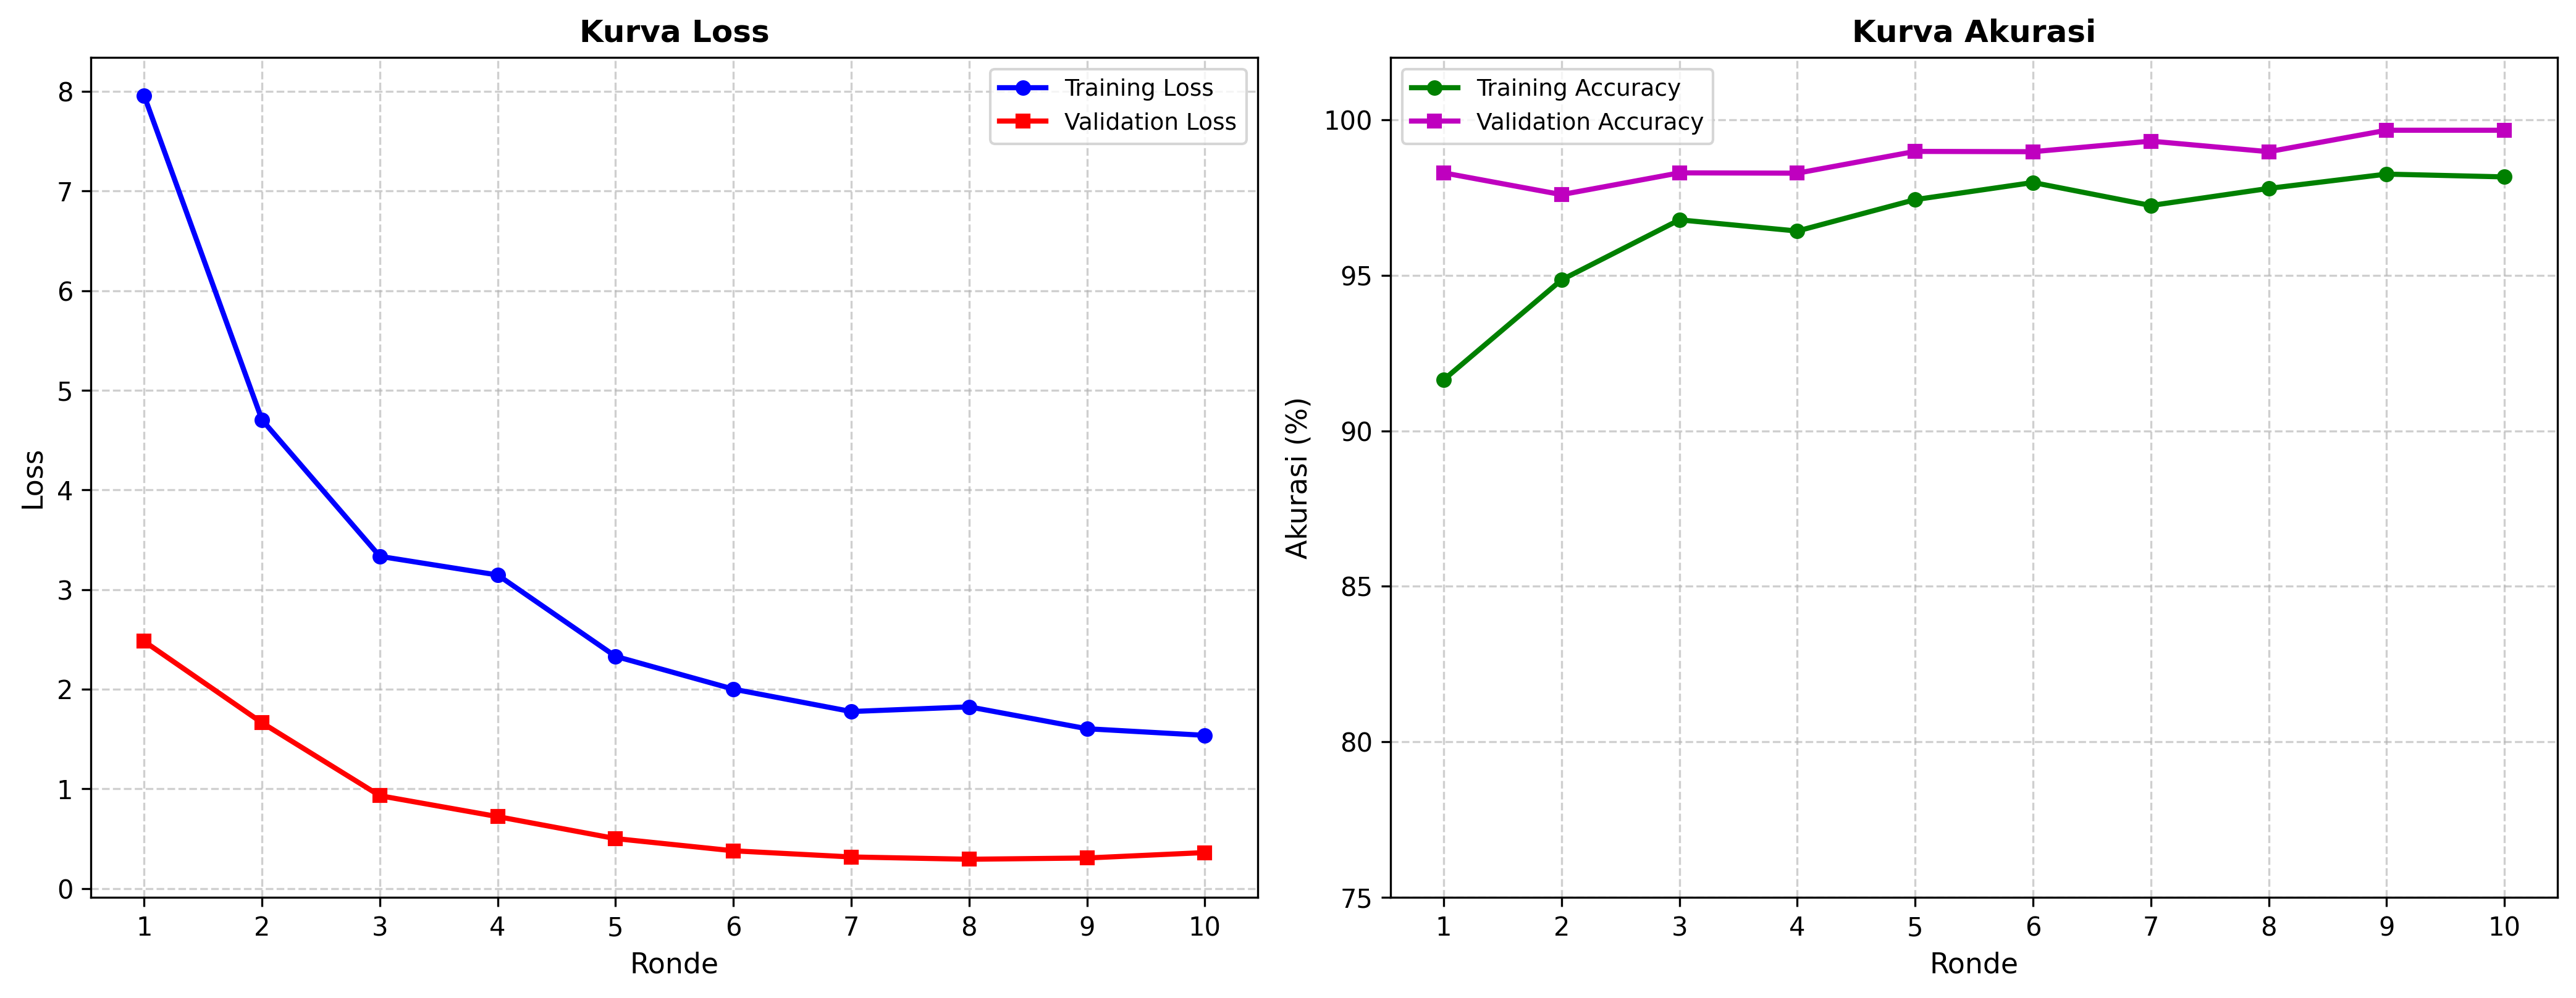
\includegraphics[width=\columnwidth]{../../core/gambar/chart_fl_server.png}
  \caption{Kurva \textit{Loss} dan Akurasi Pelatihan \textit{Federated Learning} Global (\textit{Server})}
  \label{fig:chart-fl-server}
\end{figure}

\begin{figure}[H]
  \centering
  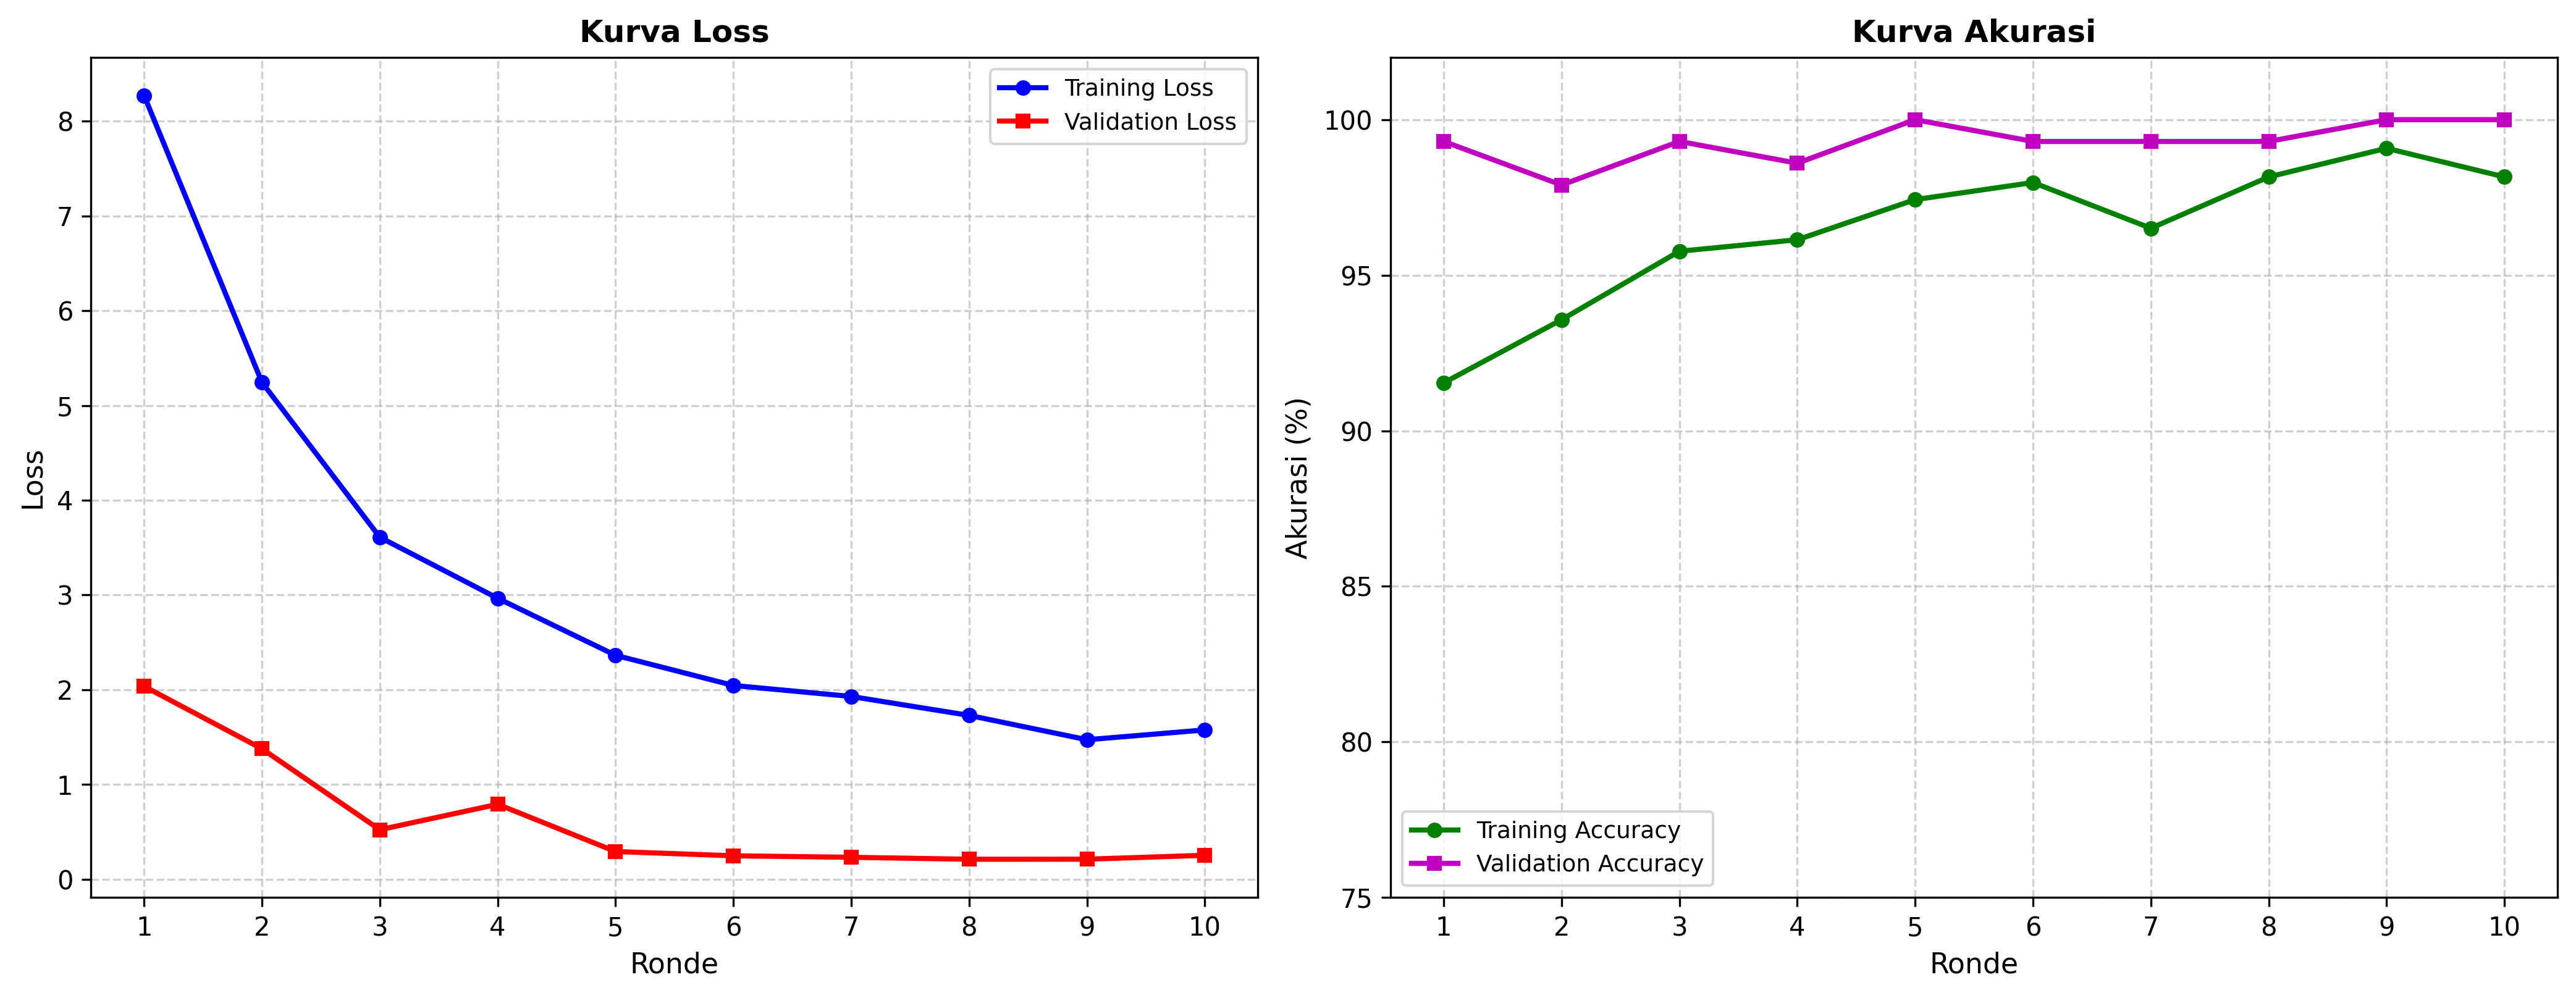
\includegraphics[width=\columnwidth]{../../core/gambar/chart_fl_client1.png}
  \caption{Kurva \textit{Loss} dan Akurasi Pelatihan \textit{Federated Learning Client} 1 (Jetson Nano)}
  \label{fig:chart-fl-client1}
\end{figure}

\begin{figure}[H]
  \centering
  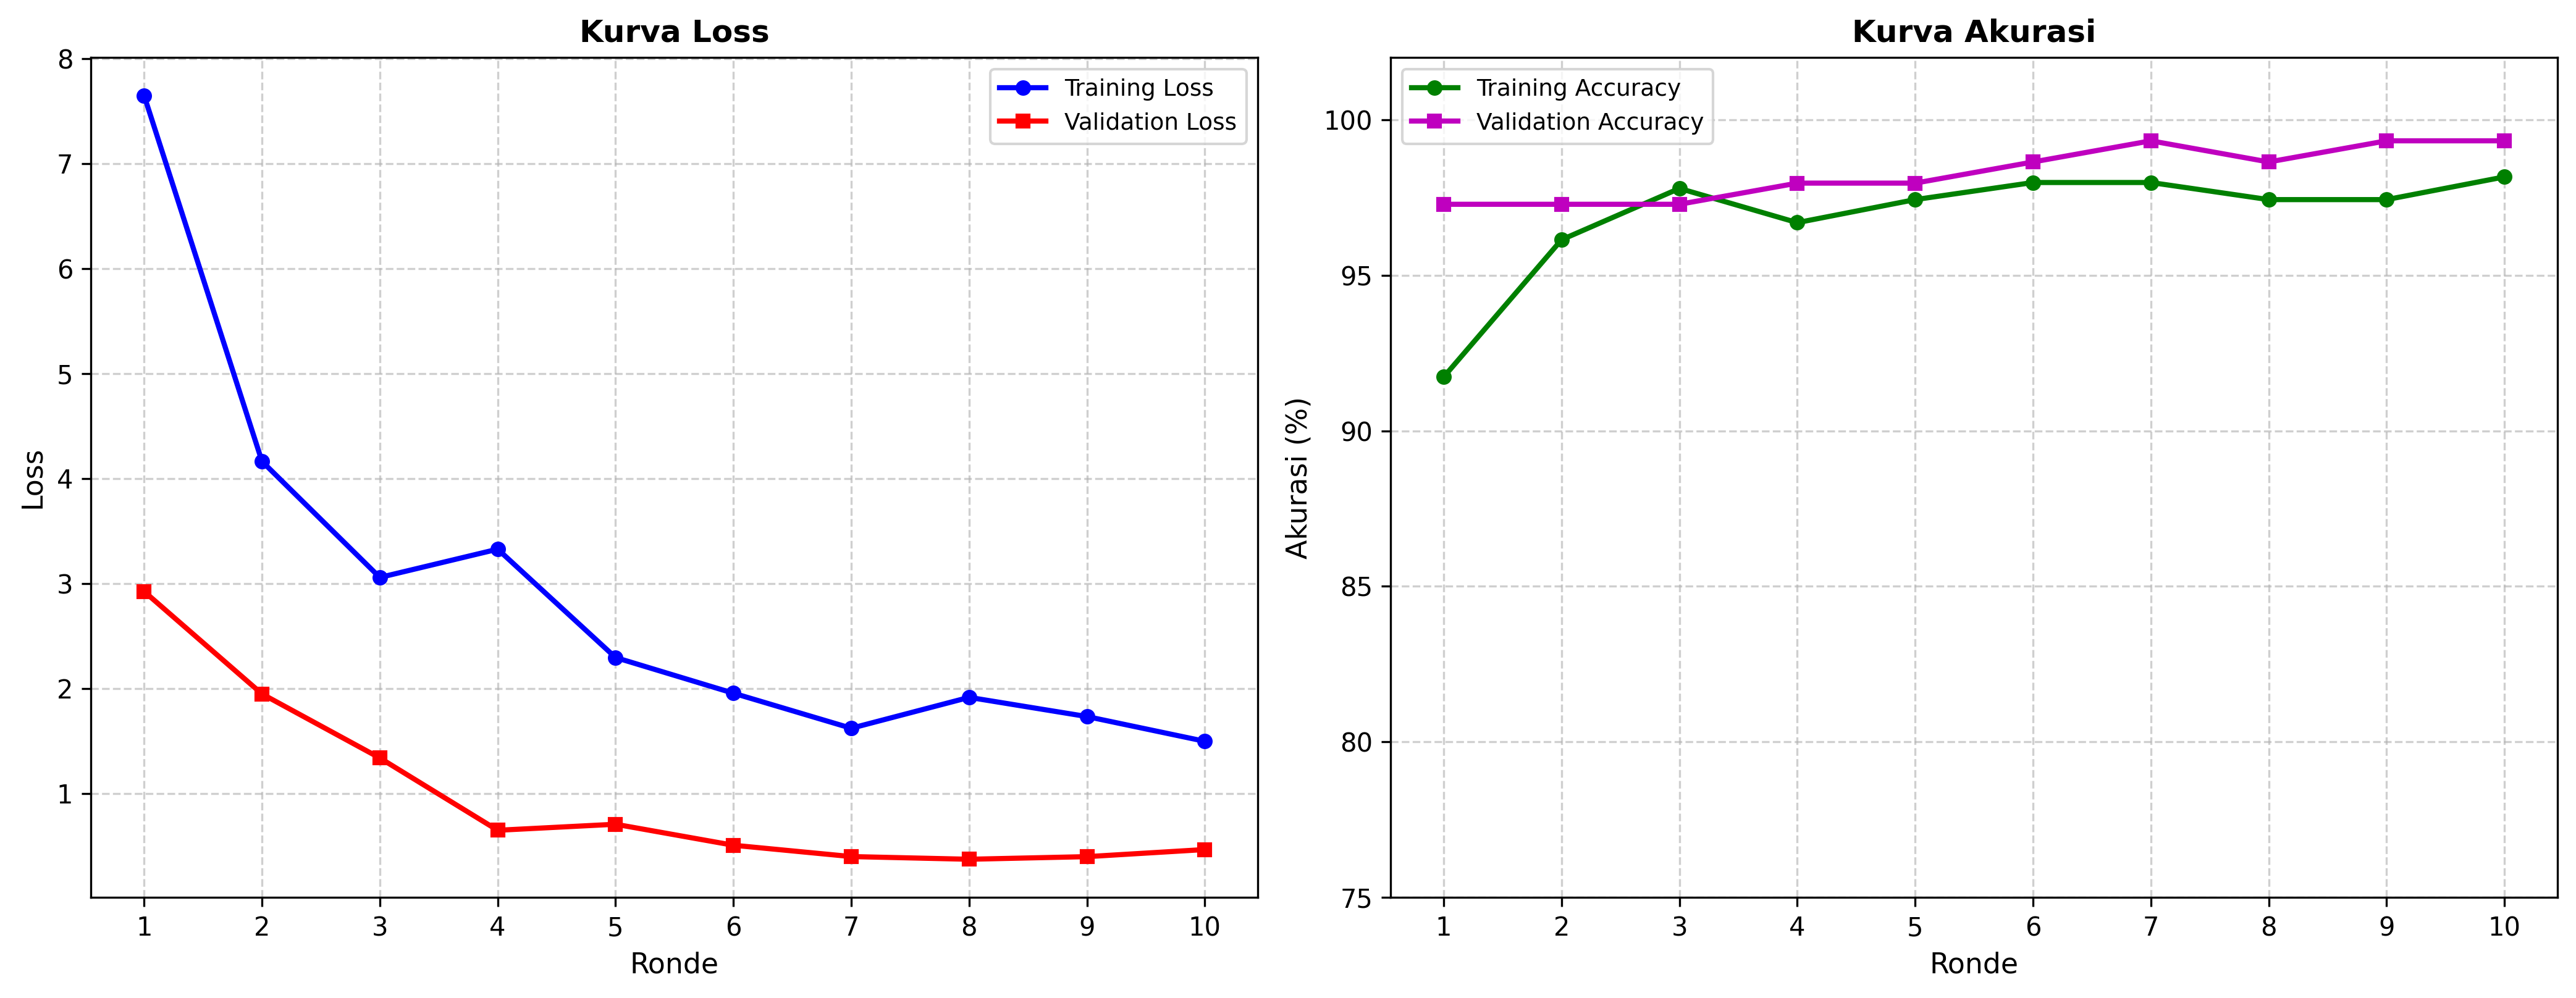
\includegraphics[width=\columnwidth]{../../core/gambar/chart_fl_client2.png}
  \caption{Kurva \textit{Loss} dan Akurasi Pelatihan \textit{Federated Learning Client} 2 (Raspberry Pi)}
  \label{fig:chart-fl-client2}
\end{figure}

\begin{figure}[H]
  \centering
  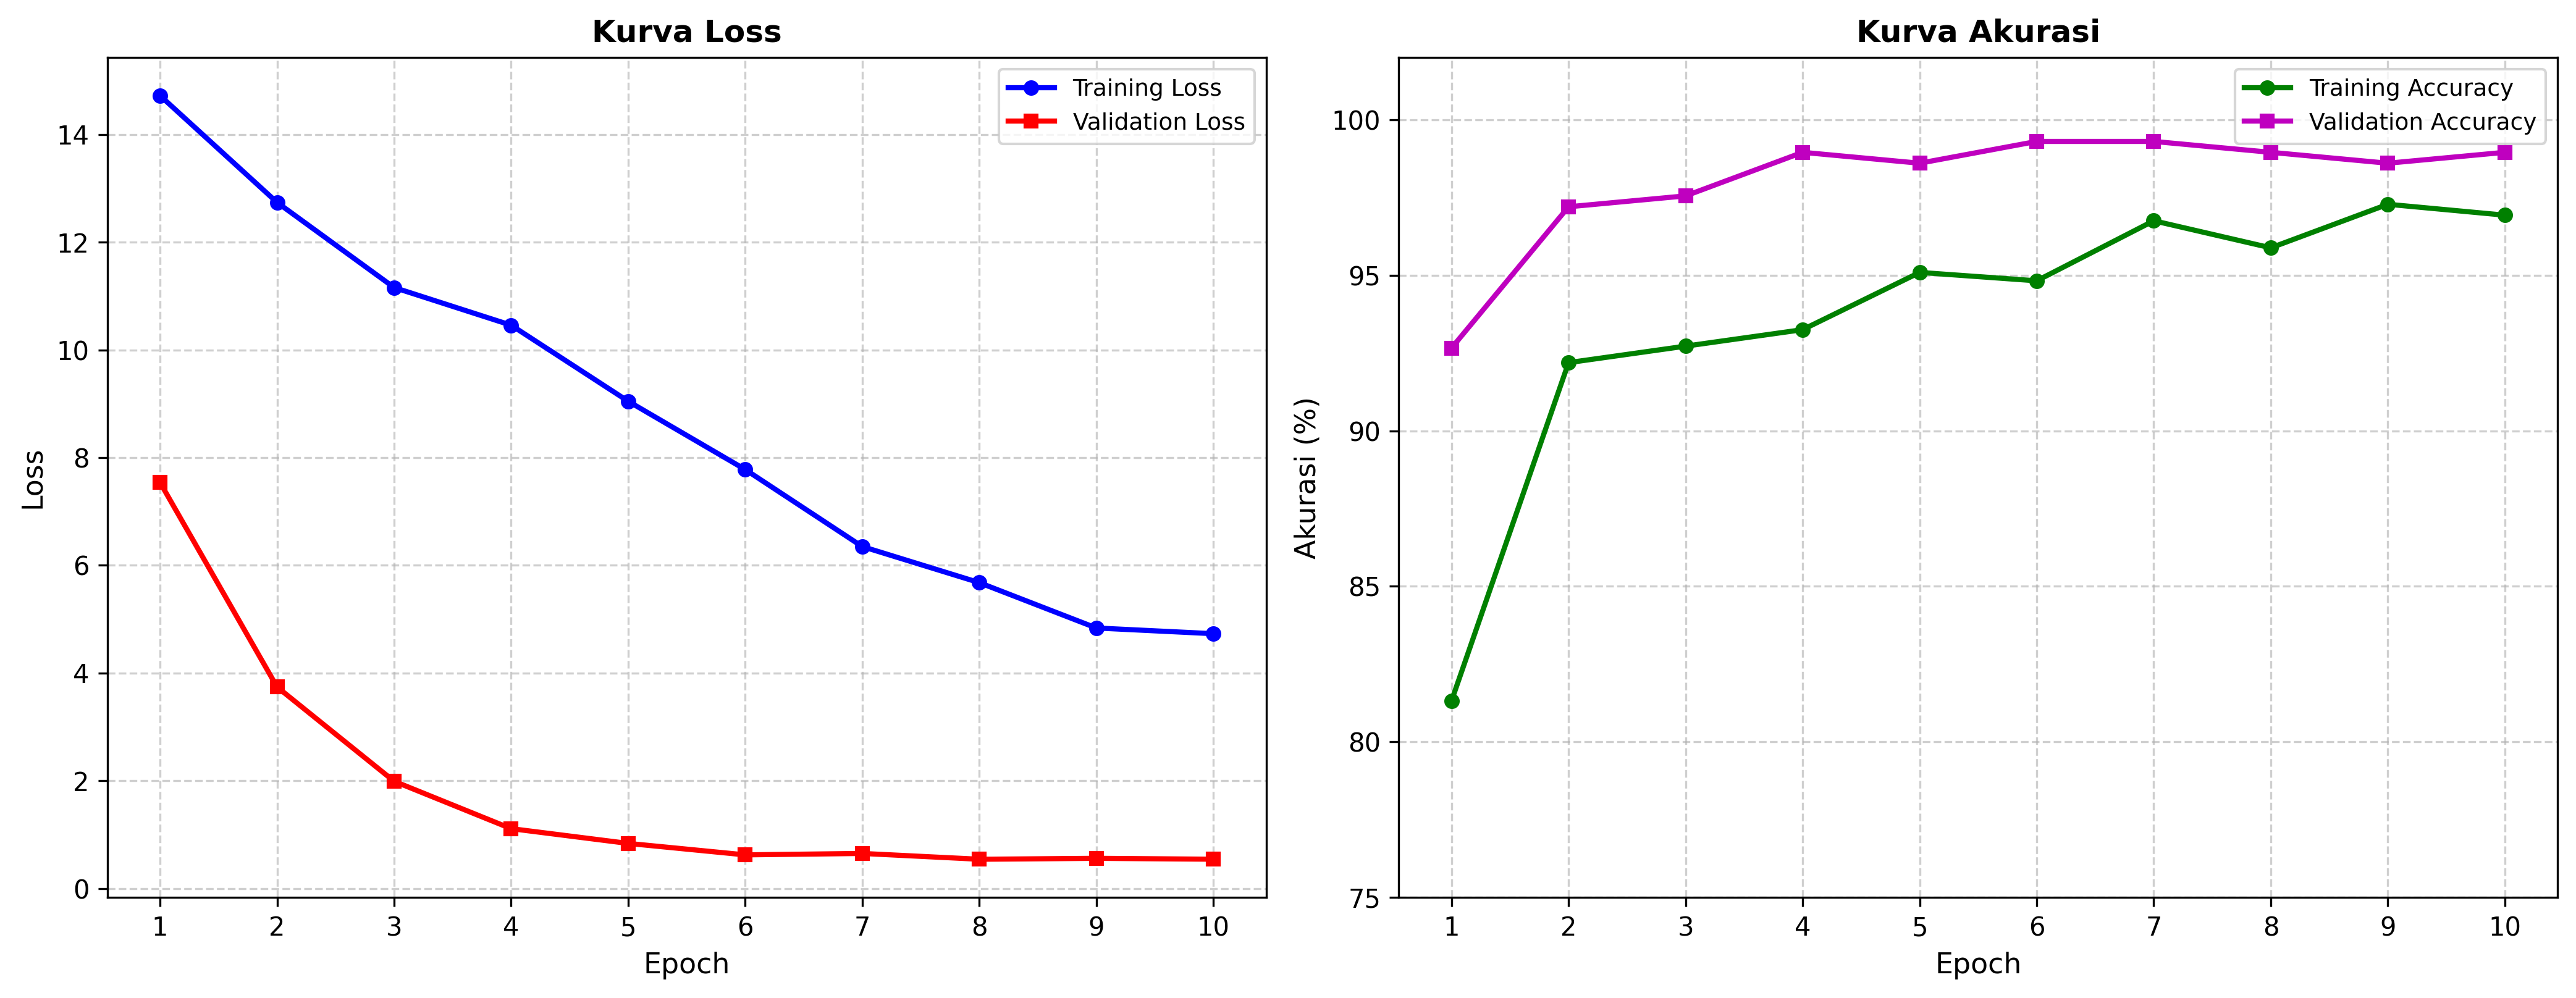
\includegraphics[width=\columnwidth]{../../core/gambar/chart_cl.png}
  \caption{Kurva \textit{Loss} dan Akurasi Pelatihan \textit{Centralized Learning}}
  \label{fig:chart-cl}
\end{figure}

Berdasarkan Tabel~\ref{tab:perbandingan-pelatihan} dan kurva pada Gambar~\ref{fig:chart-fl-server}, Gambar~\ref{fig:chart-fl-client1}, Gambar~\ref{fig:chart-fl-client2}, dan Gambar~\ref{fig:chart-cl}, kedua pendekatan menunjukkan kemampuan yang setara dalam mencapai konvergensi optimal. Model global hasil \textit{Federated Learning} mampu mencapai akurasi akhir 98,16\% (\textit{validation accuracy} 99,66\%, \textit{validation loss} 0,3599) pada ronde ke-10, sedikit mengungguli \textit{Centralized Learning} yang mencatatkan akurasi 96,93\% (\textit{validation accuracy} 98,95\%, \textit{validation loss} 0,5457) pada \textit{epoch} ke-10. Hal ini membuktikan bahwa pembagian proses pelatihan secara terdistribusi menggunakan algoritma FedProx tetap mampu menghasilkan kualitas model yang kompetitif tanpa degradasi performa yang signifikan.

Namun, sebagaimana tercantum pada Tabel~\ref{tab:perbandingan-pelatihan}, terdapat perbedaan yang sangat kontras dari segi durasi waktu pelatihan keseluruhan. Metode \textit{Federated Learning} memerlukan total durasi waktu latih yang jauh lebih lama, yaitu 5034,13 detik, dibandingkan dengan metode \textit{Centralized Learning} yang hanya memakan waktu 439,99 detik. Perbedaan ini terjadi karena pelatihan terdistribusi sangat terpengaruh oleh kecepatan perangkat paling lambat (\textit{straggler effect}). Perangkat Raspberry Pi 3 Model B (RAM 1 GB) membutuhkan waktu berkisar antara 334 hingga 384 detik per ronde, sedangkan Jetson Nano (RAM 4 GB) jauh lebih cepat dengan durasi stabil 113 hingga 114 detik per ronde, sebagaimana dirangkum pada Tabel~\ref{tab:fl-client-metrics}.

Keunggulan utama \textit{Federated Learning} terlihat jelas pada efisiensi \textit{bandwidth}. Metode terdistribusi ini hanya menghabiskan 159,46 MB sepanjang 10 ronde karena hanya mentransmisikan bobot model (\textit{weights}), berbanding terbalik dengan \textit{Centralized Learning} yang memakan 1152,34 MB karena harus mengunggah seluruh dataset citra mentah ke \textit{server} pusat. Adapun konsumsi energi \textit{Federated Learning} tercatat lebih besar (0,089481 kWh) akibat durasi pelatihan yang lama pada seluruh perangkat secara bersamaan, sedangkan \textit{Centralized Learning} hanya sebesar 0,012222 kWh.

\subsection{Pengujian Inferensi}

\subsubsection{Real-Life}
Untuk membandingkan performa secara adil antara \textit{Centralized Learning} dan terdistribusi \textit{Federated Learning}, pengujian inferensi ini dilakukan pada empat skenario konfigurasi perangkat operasional yang dirangkum pada Tabel~\ref{tab:skenario-perangkat}.

{\fontsize{8}{9}\selectfont
\begin{table}[H]
\caption{Skenario Konfigurasi Perangkat Operasional}
\begin{center}
\resizebox{\columnwidth}{!}{
  \begin{tabular}{|p{2.5cm}|p{5.5cm}|}
    \hline
    \textbf{Skenario} & \textbf{Keterangan} \\
    \hline
    \textit{Centralized Learning Client} 1 & Perangkat \textit{edge} Jetson Nano yang menjalankan model hasil \textit{Centralized Learning}. \\
    \hline
    \textit{Centralized Learning Client} 2 & Perangkat \textit{edge} Raspberry Pi yang menjalankan model hasil \textit{Centralized Learning}. \\
    \hline
    \textit{Federated Learning} A & Perangkat \textit{edge} Jetson Nano yang menjalankan model hasil \textit{Federated Learning} dengan data dari Jetson Nano (registrasi dilakukan di \textit{Client} 1 dan absensi dilakukan di \textit{Client} 1). \\
    \hline
    \textit{Federated Learning} B & Perangkat \textit{edge} Raspberry Pi yang menjalankan model hasil \textit{Federated Learning} untuk melakukan absensi (registrasi dilakukan di \textit{Client} 1 dan absensi dilakukan di \textit{Client} 2). \\
    \hline
  \end{tabular}
}
\label{tab:skenario-perangkat}
\end{center}
\end{table}
}

Pengujian inferensi nyata berfokus pada keandalan sistem dalam mengenali wajah subjek di bawah variasi jarak pemindaian dan intensitas cahaya secara langsung pada perangkat keras lokal dengan ambang kepercayaan (\textit{confidence threshold}) sebesar 0,7.

Dari segi fungsionalitas biner pada kondisi nyata (\textit{real-life}), baik model hasil \textit{Centralized Learning} maupun \textit{Federated Learning} menunjukkan keandalan yang setara. Pada kedua kondisi pencahayaan (cukup cahaya 341,01 lux dan minim cahaya 47,54 lux), seluruh skenario pengujian verifikasi kehadiran pada jarak 0,5 meter hingga 3 meter dinyatakan berhasil mendeteksi dan mengenali wajah mahasiswa secara tepat. Evaluasi lebih mendalam pada kondisi cukup cahaya menunjukkan tingkat keberhasilan klasifikasi di atas 90\% untuk seluruh skenario (93\% untuk \textit{Centralized Learning Client} 1 dan 2, 97\% untuk \textit{Federated Learning} A, serta 100\% untuk \textit{Federated Learning} B). Nilai \textit{Cosine Similarity} rata-rata yang dicapai oleh skenario \textit{Federated Learning} (0,8360 untuk \textit{Federated Learning} A dan 0,8681 untuk \textit{Federated Learning} B) juga mampu mengimbangi hasil pencapaian \textit{Centralized Learning} (0,7817 untuk \textit{Centralized Learning Client} 1 dan 0,8161 untuk \textit{Centralized Learning Client} 2). Hasil pencatatan akurasi, nilai \textit{Cosine Similarity}, serta durasi latensi pemrosesan inferensi dirangkum secara lengkap pada Tabel~\ref{tab:akurasi-cukup} dan Tabel~\ref{tab:latensi-cukup} untuk kondisi cukup cahaya, serta Tabel~\ref{tab:akurasi-minim} dan Tabel~\ref{tab:latensi-minim} untuk kondisi minim cahaya.

\begin{table}[H]
\caption{Hasil Pengujian Akurasi dan Kemiripan Kosinus (Cukup Cahaya: 341,01 lux)}
\begin{center}
\resizebox{\columnwidth}{!}{
  \begin{tabular}{|l|c|c|c|c|}
    \hline
    \multirow{2}{*}{\textbf{Skenario}} & \textbf{Akurasi} & \multicolumn{3}{c|}{\textbf{\textit{Cosine Similarity}}} \\
    \cline{3-5}
    & \textbf{(\%)} & \textbf{Rata-rata} & \textbf{Max} & \textbf{Min} \\
    \hline
    \textit{Centralized Client 1} & 93 & 0,7817 & 0,8403 & 0,6635 \\
    \textit{Centralized Client 2} & 93 & 0,8161 & 0,8925 & 0,3749 \\
    \textit{Federated Learning A} & 97 & 0,8360 & 0,9414 & 0,6785 \\
    \textit{Federated Learning B} & 100 & 0,8681 & 0,9477 & 0,7868 \\
    \hline
  \end{tabular}
}
\label{tab:akurasi-cukup}
\end{center}
\end{table}

\begin{table}[H]
\caption{Hasil Pengujian Latensi Inferensi (Cukup Cahaya: 341,01 lux)}
\begin{center}
\resizebox{\columnwidth}{!}{
  \begin{tabular}{|l|c|c|c|}
    \hline
    \textbf{Skenario} & \textbf{Rata-rata (ms)} & \textbf{Max (ms)} & \textbf{Min (ms)} \\
    \hline
    \textit{Centralized Client 1} & 724,97 & 793 & 679 \\
    \textit{Centralized Client 2} & 3094,93 & 3344 & 2881 \\
    \textit{Federated Learning A} & 764,60 & 2190 & 684 \\
    \textit{Federated Learning B} & 3172,30 & 3361 & 2942 \\
    \hline
  \end{tabular}
}
\label{tab:latensi-cukup}
\end{center}
\end{table}

\begin{table}[H]
\caption{Hasil Pengujian Akurasi dan Kemiripan Kosinus (Minim Cahaya: 47,54 lux)}
\begin{center}
\resizebox{\columnwidth}{!}{
  \begin{tabular}{|l|c|c|c|c|}
    \hline
    \multirow{2}{*}{\textbf{Skenario}} & \textbf{Akurasi} & \multicolumn{3}{c|}{\textbf{\textit{Cosine Similarity}}} \\
    \cline{3-5}
    & \textbf{(\%)} & \textbf{Rata-rata} & \textbf{Max} & \textbf{Min} \\
    \hline
    \textit{Centralized Client 1} & 97 & 0,8031 & 0,8653 & 0,5733 \\
    \textit{Centralized Client 2} & 93 & 0,8142 & 0,8898 & 0,2866 \\
    \textit{Federated Learning A} & 97 & 0,8248 & 0,9024 & 0,6799 \\
    \textit{Federated Learning B} & 90 & 0,8607 & 0,9424 & 0,6070 \\
    \hline
  \end{tabular}
}
\label{tab:akurasi-minim}
\end{center}
\end{table}

\begin{table}[H]
\caption{Hasil Pengujian Latensi Inferensi (Minim Cahaya: 47,54 lux)}
\begin{center}
\resizebox{\columnwidth}{!}{
  \begin{tabular}{|l|c|c|c|}
    \hline
    \textbf{Skenario} & \textbf{Rata-rata (ms)} & \textbf{Max (ms)} & \textbf{Min (ms)} \\
    \hline
    \textit{Centralized Client 1} & 737,23 & 799 & 678 \\
    \textit{Centralized Client 2} & 3231,83 & 3671 & 2411 \\
    \textit{Federated Learning A} & 719,13 & 766 & 680 \\
    \textit{Federated Learning B} & 3147,57 & 3328 & 2950 \\
    \hline
  \end{tabular}
}
\label{tab:latensi-minim}
\end{center}
\end{table}

Meskipun tingkat keberhasilan klasifikasi (akurasi) dari model global \textit{Federated Learning} mampu menyamai metode terpusat, terdapat perbedaan latensi inferensi yang sangat kontras di antara kedua perangkat \textit{edge}. Perangkat Jetson Nano memproses inferensi secara cepat dengan rata-rata waktu masing-masing sebesar 724,97 ms dan 764,60 ms (cukup cahaya) serta 737,23 ms dan 719,13 ms (minim cahaya). Sementara itu, Raspberry Pi membutuhkan waktu rata-rata yang jauh lebih lambat, yaitu berkisar antara 3094,93 ms hingga 3231,83 ms. Perbedaan latensi pemrosesan yang terjadi murni disebabkan oleh perbedaan spesifikasi dan kapasitas komputasi dari masing-masing unit perangkat keras lokal (khususnya kapasitas RAM).

\subsubsection{Video Simulasi}
Pengujian inferensi kontinu dilakukan menggunakan lima berkas rekaman video simulasi kehadiran mahasiswa melewati pintu yang dirangkum pada Tabel~\ref{tab:skenario-video}. Hasil pengujian disajikan pada Tabel~\ref{tab:video-deteksi} (deteksi mahasiswa), Tabel~\ref{tab:video-salah-absen} (kasus salah absen), dan Tabel~\ref{tab:video-durasi} (durasi pemrosesan).

{\fontsize{8}{9}\selectfont
\begin{table}[H]
\caption{Skenario Pengujian Video Simulasi}
\begin{center}
\resizebox{\columnwidth}{!}{
  \begin{tabular}{|p{5cm}|c|p{3.5cm}|}
    \hline
    \textbf{Sumber Video} & \textbf{Kode} & \textbf{Keterangan} \\
    \hline
    rec\_feed\_20260507\_1150\_010.mp4 & A & Terdapat 2 mahasiswa yang terdaftar tidak mengenakan kacamata. \\
    \hline
    rec\_feed\_20260519\_0957\_003.mp4 & B & Terdapat 1 mahasiswa yang terdaftar mengenakan kacamata. \\
    \hline
    rec\_feed\_20260521\_1006\_008.mp4 & C & Terdapat 2 mahasiswa yang terdaftar mengenakan kacamata. \\
    \hline
    rec\_feed\_20260526\_0956\_003.mp4 & D & Terdapat 2 mahasiswa yang terdaftar dengan 1 mahasiswa tidak mengenakan kacamata dan 1 mahasiswa mengenakan kacamata tapi saat pengambilan data tidak mengenakan kacamata. \\
    \hline
    rec\_feed\_20260526\_0956\_023.mp4 & E & Terdapat 0 mahasiswa yang terdaftar; tujuan untuk menguji ketahanan sistem terhadap kasus salah absen. \\
    \hline
  \end{tabular}
}
\label{tab:skenario-video}
\end{center}
\end{table}
}

\begin{table}[H]
\caption{Hasil Pengujian Deteksi Mahasiswa pada Video Simulasi}
\begin{center}
\resizebox{\columnwidth}{!}{
  \begin{tabular}{|c|c|c|c|c|}
    \hline
    \textbf{Skenario Video} & \textbf{\begin{tabular}[c]{@{}c@{}}Centralized\\Client 1\end{tabular}} & \textbf{\begin{tabular}[c]{@{}c@{}}Centralized\\Client 2\end{tabular}} & \textbf{\begin{tabular}[c]{@{}c@{}}Federated\\Learning A\end{tabular}} & \textbf{\begin{tabular}[c]{@{}c@{}}Federated\\Learning B\end{tabular}} \\
    \hline
    Video A & 2/2 & 2/2 & 2/2 & 2/2 \\
    \hline
    Video B & 1/1 & 1/1 & 1/1 & 1/1 \\
    \hline
    Video C & 1/2 & 1/2 & 1/2 & 1/2 \\
    \hline
    Video D & 2/2 & 2/2 & 2/2 & 2/2 \\
    \hline
    Video E & 0/0 & 0/0 & 0/0 & 0/0 \\
    \hline
  \end{tabular}
}
\label{tab:video-deteksi}
\end{center}
\end{table}

\begin{table}[H]
\caption{Hasil Pengujian Kasus Salah Absen pada Video Simulasi}
\begin{center}
\resizebox{\columnwidth}{!}{
  \begin{tabular}{|c|c|c|c|c|}
    \hline
    \textbf{Skenario Video} & \textbf{\begin{tabular}[c]{@{}c@{}}Centralized\\Client 1\end{tabular}} & \textbf{\begin{tabular}[c]{@{}c@{}}Centralized\\Client 2\end{tabular}} & \textbf{\begin{tabular}[c]{@{}c@{}}Federated\\Learning A\end{tabular}} & \textbf{\begin{tabular}[c]{@{}c@{}}Federated\\Learning B\end{tabular}} \\
    \hline
    Video A & 0 & 0 & 2 & 2 \\
    \hline
    Video B & 0 & 0 & 0 & 0 \\
    \hline
    Video C & 0 & 0 & 0 & 0 \\
    \hline
    Video D & 0 & 0 & 1 & 2 \\
    \hline
    Video E & 0 & 0 & 0 & 0 \\
    \hline
  \end{tabular}
}
\label{tab:video-salah-absen}
\end{center}
\end{table}

\begin{table}[H]
\caption{Hasil Pengujian Durasi Pemrosesan Video Simulasi (detik)}
\begin{center}
\resizebox{\columnwidth}{!}{
  \begin{tabular}{|c|c|c|c|c|}
    \hline
    \textbf{Skenario Video} & \textbf{\begin{tabular}[c]{@{}c@{}}Centralized\\Client 1\end{tabular}} & \textbf{\begin{tabular}[c]{@{}c@{}}Centralized\\Client 2\end{tabular}} & \textbf{\begin{tabular}[c]{@{}c@{}}Federated\\Learning A\end{tabular}} & \textbf{\begin{tabular}[c]{@{}c@{}}Federated\\Learning B\end{tabular}} \\
    \hline
    Video A & 835,83 & 1795,57 & 811,89 & 1790,22 \\
    \hline
    Video B & 454,28 & 1044,80 & 486,58 & 1030,19 \\
    \hline
    Video C & 364,06 & 850,78 & 392,94 & 843,67 \\
    \hline
    Video D & 553,52 & 1216,38 & 562,58 & 1201,21 \\
    \hline
    Video E & 388,20 & 888,18 & 390,55 & 878,88 \\
    \hline
  \end{tabular}
}
\label{tab:video-durasi}
\end{center}
\end{table}

Berdasarkan data pada Tabel~\ref{tab:video-durasi}, durasi pemrosesan video pada Jetson Nano (\textit{Centralized Client 1} dan \textit{Federated Learning A}) berjalan jauh lebih cepat secara konsisten dibanding Raspberry Pi. Sebagai contoh pada Video A, Jetson Nano menyelesaikan pemrosesan masing-masing dalam durasi 835,83 detik dan 811,89 detik, sementara Raspberry Pi membutuhkan waktu masing-masing hingga 1795,57 detik dan 1790,22 detik akibat keterbatasan RAM yang memicu proses \textit{memory swapping} virtual.

Analisis terhadap kasus salah absen (\textit{false acceptance}) menunjukkan adanya perbedaan karakteristik ketahanan antara kedua metode pembelajaran. Kasus salah absen terdeteksi pada Video A untuk skenario \textit{Federated Learning} A dan B yang mencatatkan 2 kasus salah absen, serta Video D yang mencatatkan 1 kasus pada \textit{Federated Learning} A dan 2 kasus pada \textit{Federated Learning} B. Sebaliknya, metode \textit{Centralized Learning} berhasil mencatatkan 0 kasus salah absen pada seluruh berkas video uji. Kasus salah absen pada \textit{Federated Learning} dipicu oleh keterbatasan model agregasi global dalam menangkap batas keputusan (\textit{decision boundary}) yang tajam pada fitur minor spesifik (seperti kemiripan subjek berkerudung), akibat tidak adanya pembagian citra wajah mentah secara langsung antarperangkat \textit{edge}.

Pada Video C, seluruh skenario pengujian hanya berhasil mencatatkan rasio deteksi sebesar 1/2 mahasiswa terdaftar. Kegagalan sistem dalam mengenali salah satu mahasiswa tersebut disebabkan oleh perubahan atribut visual subjek (penggunaan kacamata baru saat pengujian yang berbeda dengan kondisi registrasi awal).

\section{Kesimpulan dan Saran}

\subsection{Kesimpulan}
Berdasarkan hasil penelitian yang telah dilakukan, berikut merupakan kesimpulan yang didapatkan dari seluruh tahapan yang telah dilakukan:
\begin{enumerate}
    \item Sistem kehadiran berbasis pengenalan wajah menggunakan konsep \textit{Federated Learning} pada lingkungan \textit{Edge Computing} telah berhasil dibangun. Sistem ini diimplementasikan menggunakan model MobileFaceNet di dalam kontainer \textit{Docker} pada perangkat Jetson Nano (\textit{Client} 1) dan Raspberry Pi (\textit{Client} 2), dengan \textit{server} agregator terpusat. Melalui sistem ini, keamanan privasi data biometrik mahasiswa terjaga karena seluruh citra wajah mentah disimpan secara lokal di masing-masing perangkat \textit{client}, tanpa perlu dikirim ke \textit{server}.
    \item Adapun hasil perbandingan performa model antara metode \textit{Federated Learning} dan \textit{Centralized Learning} adalah sebagai berikut:
    \begin{itemize}
        \item Kecerdasan model global pada \textit{Federated Learning} mampu menyeimbangi \textit{Centralized Learning} dengan hasil akurasi sebesar 98,16\% dan \textit{validation loss} 0,3599, sedangkan \textit{Centralized Learning} menghasilkan akurasi sebesar 96,93\% dan \textit{validation loss} 0,5457.
        \item Durasi pelatihan keseluruhan pada \textit{Federated Learning} berjalan jauh lebih lambat yaitu selama 5034,13 detik dibandingkan \textit{Centralized Learning} yang hanya membutuhkan waktu 439,99 detik, akibat adanya waktu tunggu sinkronisasi parameter antar-perangkat.
        \item Kecepatan pelatihan lokal pada tingkat \textit{client} dipengaruhi oleh spesifikasi RAM, di mana Raspberry Pi membutuhkan waktu latih rata-rata 334 hingga 384 detik per ronde, sedangkan Jetson Nano jauh lebih cepat dengan durasi 113 hingga 114 detik per ronde.
        \item Penggunaan \textit{bandwidth} jaringan pada \textit{Federated Learning} jauh lebih efisien sebesar 159,46 MB dibandingkan \textit{Centralized Learning} yang menghabiskan 1152,34 MB karena harus mengunggah seluruh citra mentah ke \textit{server}.
        \item Konsumsi energi listrik pada \textit{Federated Learning} lebih besar mencapai 0,089481 kWh akibat durasi pelatihan yang lama pada seluruh perangkat, sedangkan \textit{Centralized Learning} lebih hemat yaitu sebesar 0,012222 kWh karena pemrosesan terpusat selesai secara cepat di tingkat \textit{server}.
        \item Performa inferensi secara nyata (\textit{real-life}) pada kedua metode menghasilkan tingkat keberhasilan fungsionalitas 100\% pada jarak pemindaian 0,5 meter hingga 3 meter pada kondisi cahaya cukup dan minim dengan tingkat keberhasilan klasifikasi stabil di atas 90\% pada ambang batas kepercayaan 0,7. Latensi inferensi lokal pada Jetson Nano berjalan cepat ($\sim$700 ms) sedangkan pada Raspberry Pi berjalan lambat ($\sim$3100 ms).
        \item Kecepatan proses inferensi video pada tingkat \textit{client} dipengaruhi oleh spesifikasi RAM, di mana Raspberry Pi membutuhkan waktu pemrosesan yang jauh lebih lambat (berkisar antara 843,67 hingga 1795,57 detik) sedangkan Jetson Nano jauh lebih cepat dengan durasi berkisar antara 364,06 hingga 835,83 detik.
        \item Metode \textit{Centralized Learning} lebih unggul dalam mencegah salah absen (0 kasus salah absen) dibandingkan \textit{Federated Learning} yang mengalami beberapa kasus salah absen akibat generalisasi model lokal.
        \item Terjadi kegagalan pengenalan mahasiswa pada pengujian video simulasi akibat adanya perubahan atribut visual yang tidak terdaftar saat pengambilan data latih.
    \end{itemize}
\end{enumerate}

\subsection{Saran}
Berdasarkan keterbatasan sistem serta hasil evaluasi yang diperoleh sepanjang pelaksanaan penelitian ini, beberapa saran yang dapat diajukan untuk pengembangan penelitian selanjutnya adalah sebagai berikut:
\begin{enumerate}
    \item Menggunakan arsitektur model pengenalan wajah alternatif yang lebih modern selain \textit{MobileFaceNet} guna menganalisis perbandingan akurasi dan latensi inferensinya.
    \item Menerapkan metode deteksi keaktifan wajah (\textit{anti-spoofing}) untuk memperkuat keamanan sistem dari ancaman pemalsuan identitas menggunakan foto atau video.
    \item Menggunakan perangkat keras \textit{edge} dengan spesifikasi komputasi dan kapasitas RAM yang lebih tinggi agar proses pelatihan terdistribusi dapat berjalan lebih cepat serta mampu menampung skala data latih yang lebih besar.
    \item Mengekspansi skala pengujian dengan melibatkan lebih dari 30 subjek mahasiswa untuk mengevaluasi keandalan serta skalabilitas model global hasil agregasi secara lebih luas.
\end{enumerate}

\renewcommand{\refname}{Daftar Pustaka}
\begin{thebibliography}{00}
\bibitem{b1} A. Brecko, E. Kajati, J. Koziorek, and I. Zolotova, ``Federated Learning for Edge Computing: A Survey,'' Sep. 01, 2022, MDPI. doi: 10.3390/app12189124.
\bibitem{b2} A. Nandi, F. Xhafa, and R. Kumar, ``A Docker-based federated learning framework design and deployment for multi-modal data stream classification,'' Computing, vol. 105, no. 10, pp. 2195--2229, Oct. 2023, doi: 10.1007/s00607-023-01179-5.
\bibitem{b3} N. Srinu, C. S. S. Kumar, M. Senthil, and D. B. Babu, ``Smart Attendence Recording System Utilizing CNN and Edge Computing Techniques,'' in 2025 5th International Conference on Soft Computing for Security Applications (ICSCSA), IEEE, Aug. 2025, pp. 551--558. doi: 10.1109/ICSCSA66339.2025.11170847.
\bibitem{b4} M. Sta\v{n}o, L. Hluch\'{y}, P. Krammer, and M. Hucko, ``Docker Survey for FLOps Efficiency,'' in Proceedings of the International Conference on Cybernetics and Informatics, K and I, Institute of Electrical and Electronics Engineers Inc., 2025. doi: 10.1109/KI64036.2025.10916451.
\bibitem{b5} J. Kim, T. Park, H. Kim, and S. Kim, ``Federated Learning for Face Recognition,'' in Digest of Technical Papers - IEEE International Conference on Consumer Electronics, Institute of Electrical and Electronics Engineers Inc., Jan. 2021. doi: 10.1109/ICCE50685.2021.9427748.
\bibitem{b6} M. Shaheen, M. S. Farooq, T. Umer, and B. S. Kim, ``Applications of Federated Learning; Taxonomy, Challenges, and Research Trends,'' Electronics (Switzerland), vol. 11, no. 4, Feb. 2022, doi: 10.3390/electronics11040670.
\bibitem{b7} D. J. Beutel et al., ``Flower: A Friendly Federated Learning Research Framework,'' Mar. 2022, [Online]. Available: http://arxiv.org/abs/2007.14390
\bibitem{b8} Y. Xiong, J. Cao, and G. Chen, ``Federated Learning Spam Detection Based on FedProx and Multi-Level Multi-Feature Fusion,'' Informatics, vol. 12, no. 3, Sep. 2025, doi: 10.3390/informatics12030093.
\bibitem{b9} J. Xiao, W. Wang, L. Zhang, and H. Liu, ``A MobileFaceNet-Based Face Anti-Spoofing Algorithm for Low-Quality Images,'' Electronics (Switzerland), vol. 13, no. 14, Jul. 2024, doi: 10.3390/electronics13142801.
\bibitem{b10} Xiaoccer, ``MobileFaceNet.'' Accessed: Dec. 07, 2025. [Online]. Available: https://github.com/Xiaoccer/MobileFaceNet\_Pytorch.git
\end{thebibliography}

\end{document}